\documentclass[12pt,a4paper]{article}
\usepackage[ngerman]{babel}
\usepackage[margin=2cm]{geometry}
\usepackage{amsmath}
\usepackage{amssymb}
\usepackage{graphicx}
\usepackage{tikz}
\usepackage{float}
\usepackage{hyperref}
\usepackage{cite}
\usepackage{setspace}

\onehalfspacing

\title{\Large Bewusstsein von Konsequenzen:\\
\textit{Knoten, Kanten und die Rolle des menschlichen Gehirns\\
in der Wahrnehmung natürlicher Ordnungssysteme}}

\author{Verfasser}
\date{\today}

\begin{document}

\maketitle

\begin{abstract}
Diese Arbeit untersucht die zentrale These, dass Menschen durch mangelndes Bewusstsein ihrer Handlungskonsequenzen ihrer eigenen Entwicklung im Weg stehen. Unter Anwendung von Graphentheorie (Knoten und Kanten), Neurowissenschaften und Philosophie wird argumentiert, dass die Natur durch konstante Systeme (Sonne, Gravitation, feste Bodenordnung) permanente Konsequenzmechanismen demonstriert. Das menschliche Gehirn, konzeptualisiert als Zustandsübergangsmaschine, wird analysiert, um zu verstehen, wie Bewusstseinsdefizite und mangelnde Konsequenzbewusstheit zu suboptimalem Handeln und zur Selbstblockade führen. Die zentrale Erkenntnis der Arbeit ist, dass der Mensch sich selbst im Wege steht, nicht weil die Konsequenzen seines Handelns verborgen sind, sondern weil er sich ihrer nicht bewusst ist oder sie nicht bewusst wahrnehmen möchte.
\end{abstract}

\section{Einleitung}

Die menschliche Existenz ist geprägt durch ein grundlegendes Paradoxon: Der Mensch verfügt über eine beispiellose Kapazität für Bewusstsein, Reflexion und Vorausschau, nutzt diese Fähigkeiten jedoch oft nicht, um sich selbst aus dem Weg zu gehen. Dieses Phänomen der Selbstblockade manifestiert sich in einer alltäglichen Realität, in der Menschen ihre Ziele verfolgen, diese aber durch mangelndes Verständnis oder mangelndes Bewusstsein der Konsequenzen ihrer eigenen Handlungen gehindert werden \cite{jonas2003prinzip}. Diese paradoxe Situation ist nicht das Ergebnis mangelnder Intelligenz, sondern vielmehr das Resultat einer fundamentalen Diskrepanz zwischen der theoretischen Fähigkeit des Menschen, Konsequenzen zu verstehen, und seiner praktischen Unfähigkeit oder Unwilligkeit, sich dieser Konsequenzen bewusst zu sein.

Diese Arbeit postuliert eine radikale These: Die natürliche Welt kann als ein kohärentes, deterministisches System von Konsequenzabläufen konzeptualisiert werden, in dem jede Aktion, jede Bewegung und jede Veränderung unmittelbare und unvermeidliche Folgen mit sich bringt. Im Gegensatz dazu operiert der Mensch häufig unter der impliziten Annahme, dass seine Handlungen folgenlos sein könnten oder dass Konsequenzen auf andere, nicht auf ihn selbst, fallen werden. Der Mensch steht sich oft selbst im Weg deshalb, weil er sich der Konsequenzen seines Handelns nicht bewusst ist oder sie nicht möchte. 

Es gibt jedoch in der Natur viele Zeugen der Konsequenz, die konstant und unvermeidlich demonstrieren, dass dieses Denken fehlgeleitet ist. Die Sonne scheint immer, unabhängig davon, ob Menschen ihre Existenz beachten oder nicht. Die Erdanziehungskraft wirkt immer, überall, und verhandelt nicht mit denen, die gegen sie protestieren. Der Boden der Erde ermöglicht durch seine Ordnung das geordnete Treffen der Menschen und Stehen von Gegenständen nur so, dass es nutzbar wird. Diese naturalen Systeme sind nicht nur Metaphern, sondern konkrete, physikalische Manifestationen eines fundamentalen Prinzips: In der Natur gibt es keine Ausnahmen von Konsequenzen.

Das zentrale Argument dieser Arbeit lautet: \textit{Wo die Natur konstante Konsequenzen durchsetzt, wo sie permanente Konsequenzmechanismen demonstriert, versagt das menschliche Bewusstsein oft, diese wahrzunehmen und sie in sein Handeln zu integrieren.} Der Mensch hat das Vermögen, die Sprache der Natur zu verstehen — die Sprache von Ursache und Wirkung, von Handlung und Folge — doch er nutzt dieses Vermögen nicht, oder er verdrängt es aktiv, um sich von den Implikationen seiner Handlungen zu befreien.

Die vorliegende Arbeit ist strukturiert als eine systematische Untersuchung dieser These. Sie beginnt mit den theoretischen Grundlagen, wobei Graphentheorie als Modell für Kausalität und Konsequenzen verwendet wird. Darauf folgt eine detaillierte Analyse des menschlichen Gehirns als Zustandsübergangsmaschine, mit besonderem Fokus darauf, wie neurologische Prozesse zu Konsequenzbewusstseins-Defiziten führen können. Dann werden natürliche Systeme — insbesondere die Sonne, die Gravitation und die materiale Ordnung des Bodens — als konkrete Zeugen der Konsequenz untersucht. Die Arbeit analysiert sodann die fundamentale Asymmetrie zwischen natürlichen und menschlichen Systemen, um schließlich mit praktischen und theoretischen Implikationen für menschliches Verhalten und Entwicklung abzuschließen.

\section{Theoretische Grundlagen: Knoten, Kanten und Kausalität}

\subsection{Graphentheoretisches Modell der Wirklichkeit}

Die moderne Wissenschaft hat eine mächtige Erkenntnis gewonnen: Komplexe Systeme — egal ob sie biologischer, physikalischer oder sozialer Natur sind — können durch mathematische Strukturen modelliert werden, die als Graphen bekannt sind \cite{barabasi2002linked}. Diese Erkenntnis ist nicht bloß mathematisch von Interesse, sondern bietet eine fundamentale neue Perspektive auf die Struktur der Wirklichkeit selbst. Insbesondere erlaubt die Graphentheorie uns, Kausalität, Konsequenzen und die Vernetzung von Ereignissen auf eine Weise zu verstehen, die der tatsächlichen Struktur der Realität entspricht.

Ein Graph $G$ wird formal definiert als ein geordnetes Paar von zwei Mengen:

\begin{equation}
G = (V, E), \quad \text{wobei } V = \{v_1, v_2, \ldots, v_n\} \text{ Knoten und } E = \{e_1, e_2, \ldots, e_m\} \text{ Kanten sind}
\end{equation}

Diese abstrakte mathematische Definition hat jedoch tiefgreifende Implikationen für unser Verständnis der Wirklichkeit. In der Interpretation dieser Arbeit repräsentieren die verschiedenen Komponenten eines Graphen nicht nur mathematische Abstraktionen, sondern konkrete Aspekte der menschlichen Erfahrung und des natürlichen Handelns.

Die Knoten ($V$) repräsentieren Zustände, Ereignisse oder Handlungen. Ein Knoten könnte beispielsweise eine Entscheidung darstellen, die ein Mensch trifft, oder einen physikalischen Zustand in der Welt. Jeder Knoten ist ein diskreter Moment oder Punkt in der kontinuierlichen Wirklichkeit, ein Zustand, der vom vorherigen unterschieden werden kann. Die Kanten ($E$) sind die kritischen Verbindungen zwischen diesen Knoten und repräsentieren kausale Beziehungen oder die Konsequenzen einer Aktion. Eine Kante ist der unmittelbare Übergang von einem Zustand zu einem anderen, die unvermeidliche Linie, die Ursache mit Wirkung verbindet. Die Kantengewichte schließlich repräsentieren die Stärke oder Unmittelbarkeit einer Konsequenz — manche Konsequenzen sind sofort und unvermeidlich, während andere verzögert oder durch Zufallsfaktoren moduliert werden könnten.

Ein konkretes Beispiel veranschaulicht diese abstrakte Struktur:

\begin{equation}
v_{\text{Handlung}} \xrightarrow{e_{\text{Konsequenz}}} v_{\text{Folge}}
\end{equation}

Wenn ein Mensch beispielsweise die Handlung setzt, den Arm zu erheben und ihn dann loszulassen, dann folgt unmittelbar die Konsequenz, dass der Arm nach unten fällt — nicht weil es eine Option gibt, nicht weil es verhandelt werden könnte, sondern weil die Gravitation eine unvermeidliche Kante ist, die die Knoten »gehobener Arm« und »fallender Arm« verbindet.

Die zentrale Einsicht ist nun die folgende: Die natürliche Welt operiert als ein hochkonnektiertes, deterministisches Graphensystem, in dem jede Handlung unvermeidlich zu Konsequenzen führt. Es gibt keine isolierten Knoten in der Natur, keine Handlungen ohne Kanten, keine Ursachen ohne Wirkungen. Dies ist nicht eine metaphorische oder philosophische Aussage, sondern eine Beschreibung der tatsächlichen Struktur der physikalischen Realität. Die Physik hat dies seit Newton verstanden: Jede Kraft führt zu einer Gegenkraft, jede Aktion zu einer Reaktion. Die Natur ist, in diesem graphentheoretischen Sinne, ein vollständig verbundenes System.

\subsection{Determinismus und Bewusstsein: Die Unvermeidlichkeit von Konsequenzen}

Die natürliche Welt operiert nach Prinzipien, die keine Ausnahmen, keine Verhandlungen und keine Umgehungen zulassen. Das Universalgesetz der Gravitation, welches von Isaac Newton formuliert wurde, ist nicht ein Vorschlag oder eine Richtlinie, die unter bestimmten Umständen ignoriert werden könnte. Es ist ein absolutes, deterministisches Gesetz:

\begin{equation}
F = G \frac{m_1 m_2}{r^2}
\end{equation}

Diese Gleichung besagt, dass zwischen zwei Massen $m_1$ und $m_2$, getrennt durch eine Distanz $r$, eine Kraft $F$ wirkt, die proportional zum Produkt der Massen ist und umgekehrt proportional zum Quadrat ihrer Entfernung. Dies ist nicht eine statistische Tendenz oder eine durchschnittliche Erwartung — es ist eine absolute Beschreibung dessen, was in der Welt geschieht. Wenn ein Mensch einen Stein fallen lässt, wird er nicht »wahrscheinlich« fallen. Er wird fallen, weil die Gravitation keine Optionen bietet.

Diese mathematisch formulierte Unvermeidlichkeit der Natur steht in schärfstem Kontrast zum typischen menschlichen Verhalten und zu den kognitiven Mustern, die das menschliche Denken über Konsequenzen prägen. Der menschliche Verstand ist oft geprägt durch illusionäre Annahmen, die die tatsächliche Struktur von Ursache und Wirkung verzerren. Ein Mensch sagt sich selbst: »Mir wird schon nichts passieren«, als ob die Gesetze der Physik, der Biologie oder der Psychologie für ihn eine Ausnahme machen würden. Ein anderer Menschen sagt: »Das trifft nur andere«, als ob die Konsequenzen seiner Handlung selektiv auf andere Menschen wirken könnten, während er selbst geschützt wäre. Noch andere denken: »Diesmal wird es anders sein«, als ob das Universum sich für sie ändern würde.

Diese kognitiven Verzerrungen, diese fundamentalen Missverständnisse über die Natur von Konsequenzen, entstehen nicht aus Dummheit oder Ignoranz, sondern aus einer tiefer liegenden neurologischen und psychologischen Realität: Sie entstehen durch eine unvollständige neuronale Kartographie der Kausalzüge, durch ein Gehirn, das die Graphenstruktur der Wirklichkeit nicht vollständig erfasst hat oder erfassen will. Das menschliche Gehirn, dieses wunderbare Organ der Reflexion und des Bewusstseins, ist gleichzeitig ein Filter, der die volle Realität von Konsequenzen dämpft, verschleiert und verzerrt. Der Mensch sieht nicht die vollständige Graphenstruktur seiner Welt. Er sieht nur fragmentarische Schnipsel, unvollständige Kausalzüge, und vor allem sieht er nicht die Kanten, die seine eigenen Handlungen mit ihren Konsequenzen verbinden.

\section{Das Gehirn als Zustandsübergangsmaschine}

\subsection{Neurologische Architektur der Konsequenzwahrnehmung}

Das menschliche Gehirn, trotz seiner biologischen Komplexität und seiner organischen Natur, kann in seiner grundlegendsten Funktion als ein System von diskreten Zustandsübergängen modelliert und verstanden werden. Dies ist keine Reduktion des Gehirns auf eine bloße Maschine, sondern vielmehr eine präzise mathematische Beschreibung dessen, was das Gehirn tatsächlich tut: Es nimmt einen gegenwärtigen Zustand wahr, integriert Informationen, und geht in einen neuen Zustand über.

Ein neurologischer Zustand $s_t$ zum Zeitpunkt $t$ kann formal beschrieben werden als:

\begin{equation}
s_{t+1} = f(s_t, a_t, e_t)
\end{equation}

Diese elegante Gleichung kodiert die Essenz des neurologischen Geschehens. Der Zustand zum nächsten Zeitpunkt ($s_{t+1}$) ist eine Funktion des gegenwärtigen Zustands ($s_t$), einer Handlung, die der Mensch durchführt oder plant ($a_t$), und externer Umweltfaktoren, die auf ihn einwirken ($e_t$). Die Funktion $f$ selbst repräsentiert die neurologische Verarbeitungskette — die Neuronen, Synapsen, Neurotransmitter und die komplexen Feedback-Schleifen, die das Gehirn durchziehen.

Aber hier liegt eine entscheidende Erkenntnis: Der gegenwärtige Zustand und die unmittelbare nächste Aktion sind nicht genug. Um erfolgreich in einer kausal-konsequenziellen Welt zu agieren, um sich nicht selbst im Wege zu stehen, muss das Gehirn in der Lage sein, nicht nur einen Schritt in die Zukunft zu projizieren, sondern viele Schritte. Ein optimales Verhalten erfordert, dass das Gehirn eine vorausschauende Modellierung durchführt, eine imaginäre Simulation dessen, was passieren wird, wenn eine bestimmte Handlung durchgeführt wird.

Dies wird formal ausgedrückt als:

\begin{equation}
s_{t+n} = f^n(s_t, a_t, e_t) \quad \text{für } n > 1
\end{equation}

Diese Gleichung besagt: Der Zustand $n$ Zeitschritte in die Zukunft ist das Ergebnis der wiederholten Anwendung der Übergangsfunktion $f$ auf den gegenwärtigen Zustand, die Handlung und die Umweltfaktoren, über $n$ Iterationen hinweg. Mit anderen Worten, das Gehirn muss mental mehrere Schritte in die Zukunft gehen können. Es muss die Kette von Konsequenzen sehen können, nicht nur die unmittelbare nächste Konsequenz, sondern auch die Konsequenzen der Konsequenzen.

Dies ist die Wurzel des Problems: Das menschliche Gehirn ist oft nicht in der Lage oder nicht willens, diese extended foresight zu praktizieren. Es operiert auf kurzfristige Optimierung, auf immediate rewards und immediate threats. Es ver mag es nicht oder will nicht, die vollständige Sequenz von Zustandsübergängen zu simulieren, die aus einer Handlung folgen. Ein Raucher weiß abstrakt, dass Rauchen zu Lungenkrebs führen kann, aber sein Gehirn simuliert nicht vollständig die Sequenz: Rauchen → toxische Substanzen in der Lunge → Zellschäden → Tumorbildung → Schmerz, Atemnot, Tod. Wenn das Gehirn diese Sequenz vollständig simulierte, würde der Widerstand gegen die Handlung viel stärker sein.

\subsection{Die Konsequenzbewusstseins-Defizit (KBD): Eine quantitative Messung der Selbstblockade}

Viele Menschen leiden unter dem, was diese Arbeit das \textit{Konsequenzbewusstseins-Defizit (KBD)} nennt. Dies ist nicht eine psychiatrische Störung in dem klassischen Sinne, sondern vielmehr eine strukturelle Diskrepanz zwischen der Menge und Intensität der tatsächlich existierenden Konsequenzen einer Aktion und dem Umfang, in dem diese Konsequenzen vom handelnden Menschen bewusst wahrgenommen und in sein Entscheidungskalkül integriert werden. Das KBD kann formal quantifiziert werden:

\begin{equation}
\text{KBD} = 1 - \frac{\text{Anzahl wahrgenommener Konsequenzen}}{\text{Anzahl tatsächlicher Konsequenzen}}
\end{equation}

Diese elegante Formel erlaubt es uns, den Grad der Selbstblockade zu messen. Wenn ein Mensch beispielsweise eine Handlung durchführt, die objektiv zehn verschiedene Konsequenzen hat, aber er bewusst nur drei von ihnen wahrnimmt, dann hat er ein KBD von 0.7. Das bedeutet, dass siebzig Prozent der Konsequenzen seiner Handlung seinem bewussten Geist entgehen. Siebzig Prozent der Realität, in die er durch sein Handeln eintritt, ist für ihn unsichtbar. Dies ist nicht bloß ein Problem der Information oder des Wissens — es ist ein Problem der Wahrnehmung, der Bewusstseinsfähigkeit selbst.

Warum entsteht dieses Defizit? Die Antworten sind vielfältig und greifen tief in die neurologische, kognitive und emotionale Struktur des menschlichen Gehirns ein:

Erstens führt eine reduzierte Vorausschau zu diesem Defizit. Das Gehirn eines Menschen kann, unter idealen Bedingungen, mehrere Schritte in die Zukunft projizieren und die Kette von Konsequenzen visualisieren. In der Praxis jedoch projiziert das menschliche Gehirn oft nur einen oder zwei Schritte voraus. Es sieht die unmittelbare Konsequenz einer Handlung, aber nicht die Konsequenzen der Konsequenzen. Ein Student nimmt sich vor, »später« zu studieren statt jetzt, und sieht die unmittelbare Konsequenz: mehr Freizeit heute. Aber er sieht nicht die längerkettigen Konsequenzen dieser Entscheidung: Das Wissen von morgen wird weniger sein, die Prüfung wird schwächer ausfallen, die Chancen auf dem Arbeitsmarkt werden geringer, die finanzielle Stabilität wird unsicherer. Diese erweiterten Konsequenzen sind für ihn unsichtbar, weil sein Gehirn sie nicht projiziert.

Zweitens entstehen kognitive Verzerrungen, die das KBD verstärken. Das menschliche Denken ist strukturell verzerrt — nicht wegen eines Fehlers in der Hardware des Gehirns, sondern wegen evolutionärer Mechanismen, die sich unter anderen Bedingungen entwickelt haben. Der Bestätigungsfehler führt dazu, dass Menschen nur solche Informationen über Konsequenzen wahrnehmen und erinnern, die ihre bereits bestehenden Überzeugungen bestätigen. Der Optimismus-Bias lässt Menschen denken, dass sie selbst weniger anfällig für negative Konsequenzen sind als andere. Ein Mensch weiß intellektuell, dass Autofahren gefährlich ist, aber denkt unbewusst: »Ich bin ein guter Fahrer, mich wird es nicht treffen.« Diese kognitiven Verzerrungen sind nicht Willenschwäche, sondern strukturelle Merkmale des menschlichen Verstandes.

Drittens führt emotionale Überlagerung zur Reduktion des Konsequenzbewusstseins. Unmittelbare Triebe, Begierden und Gefühle überlagern und überschreiben langfristige, intellektuelle Verständnis von Konsequenzen. Ein Hungernder sieht einen Apfel und nimmt ihn — die unmittelbare Befriedigung überlagert jede intellektuelle Überlegung über Eigentum und Gesetz. Ein verliebter Mensch ignoriert die Konsequenzen eines untreuen Handelns, weil die emotionale Erregung des Moments stärker ist als das Verständnis der zerstörerischen Konsequenzen für die Beziehung. Diese emotionale Überlagerung ist nicht ein Mangel, sondern ein Feature des menschlichen Gehirns — es erlaubt uns, schnell zu handeln, wenn es notwendig ist. Aber in einer Welt, in der viele Konsequenzen verzögert sind und viele Handlungen Zeit haben, überlegt zu werden, wird diese Eigenschaft zum Defekt.

Viertens führt soziale Desensibilisierung dazu, dass Konsequenzen, die andere Menschen treffen, abstrakt und daher unwirklich erscheinen. Ein Mensch kann statistisch verstehen, dass ein Atomkraftwerk zehn Tode pro Jahr verursacht, aber diese zehn Tode sind abstrakt, statistisch, nicht real. Wenn jedoch eine Person, die man kennt, durch das Kraftwerk stirbt, wird die Konsequenz plötzlich konkret und real. Dies ist ein neurologisches Feature: Unser Gehirn verarbeitet konkrete, nahestehende Konsequenzen viel intensiver als abstrakte, ferne Konsequenzen. Ein Politiker kann für eine Politik stimmen, die Millionen in fernen Ländern schädigen wird, während er zögert, einen armen Menschen in seiner Nachbarschaft zu ignorieren. Die Konsequenzen für die Millionen sind zu abstrakt, zu weit entfernt.

\section{Natürliche Zeugen der Konsequenz}

\subsection{Die Sonne: Konstante Aktion und unvermeidliche Wirkung}

Die Sonne steht am Himmel — nicht metaphorisch, sondern physikalisch, eine riesige Kugel aus Plasma, 1.4 Millionen Kilometer im Durchmesser, 150 Millionen Kilometer entfernt, und sie scheint. Sie scheint jeden Tag, jede Nacht (für die eine Hälfte der Erde), jede Sekunde, seit vier Milliarden Jahren, und wird es weitere fünf Milliarden Jahre tun. Die Sonne ist das primäre Paradigma der unvermeidlichen Konsequenz im kosmischen Sinne.

Die Sonne ist ein Perpetuum mobile der Konsequenzen. Dass sie scheint, ist nicht ihre »Handlung« im menschlichen Sinne — die Sonne wählt nicht, ob sie scheinen will oder nicht. Vielmehr ist das Scheinen der Sonne das unvermeidliche Resultat ihrer inneren Struktur: der Fusionsprozess in ihrem Kern, in dem Wasserstoff in Helium umgewandelt wird und dabei enorme Energien freisetzt. Diese Energien breiten sich aus, durchstrahlen die Millionen Kilometer Raum zwischen Sonne und Erde, und wenn sie auf der Erde ankommen, produzieren sie die fundamentalsten Konsequenzen für alles Leben.

Die Energiestrahlung der Sonne kann mathematisch beschrieben werden als:

\begin{equation}
E = \frac{L_{\odot}}{4\pi r^2} \quad \text{(Energiestrom pro Flächeneinheit)}
\end{equation}

Hier ist $L_{\odot}$ die Leuchtkraft der Sonne (die totale Energiemenge, die sie pro Sekunde ausstrahlt), und $r$ ist die Entfernung von der Sonne. Die Gleichung zeigt, dass der Energiestrom pro Flächeneinheit umgekehrt proportional zum Quadrat der Entfernung ist — ein grundlegendes Gesetz, das die Sonne in keine Verhandlung verwickelt. Die Energie ist einfach da, im Raum, wirkend, konsequenzbringend.

Die Sonne demonstriert mehrere fundamentale Eigenschaften von Konsequenzen:

Erstens die Unvermeidlichkeit: Die Sonne scheint immer. Es gibt keine Umgehung, keinen Weg, ihrer Strahlung zu entkommen (außer in einem unterirdischen Bunker, aber selbst das ist nur eine Verschiebung, nicht eine echte Flucht). Ein Mensch kann protestieren, kann argumentieren, kann sich weigern — aber die Sonne scheint trotzdem. Die Sonne verhandelt nicht. Sie hört nicht auf die Einwände derer, die von ihrer Strahlung verbrannt werden. Sie hört nicht auf die Wünsche derer, die in Dunkelheit leben würden. Sie scheint, und punkt. Dies ist die ultimative Unvermeidlichkeit von Konsequenzen: Sie kümmern sich nicht um deine Einwände.

Zweitens die Universalität: Jeder Organismus auf der Erde unterliegt der Strahlung der Sonne. Keine Kreatur, keine Pflanze, kein Tier, kein Mensch kann dieser Realität entgehen. Der reiche Mensch in seinem Palast, der arme Mensch in seiner Hütte, beide sind dem Licht der Sonne unterworfen. Dies ist ein Grundprinzip: Konsequenzen sind demokratisch. Sie kümmern sich nicht um Rang, Status oder Reichtum. Ein Milliardär kann nicht schneller fallen als ein Bettler, wenn beide von einer Klippe springen. Die Gravitation kennt keine Unterschiede zwischen den Menschen.

Drittens die Kausalität: Die Strahlung der Sonne führt direkt zu eine Vielzahl von Konsequenzen — biologischen, chemischen, physikalischen. Das Pflanzenwachstum ist direkt eine Konsequenz der Photosynthese, die durch Sonnenlicht angetrieben wird. Die Zirkulation von Wärme in der Atmosphäre, die Wetterzyklen, die Jahreszeiten — alles ist eine direkte Konsequenz der Sonneneinstrahlung. Die biologischen Prozesse, die das Leben antreiben, die Stoffwechsel jeder einzelnen Zelle, die Energie in jedem Muskel — alles stammt letztlich von der Sonne. Der Mensch isst Nahrung, die von Pflanzen stammt, die vom Sonnenlicht wachsen. Der Mensch verbrennt Kohle und Öl, die fossile Energie der antiken Sonne sind. Jeder Atemzug eines Menschen, jede Bewegung eines Menschen, ist ultimativ angetrieben von der Sonne. Dies ist Kausalität im tiefsten Sinne — nicht kausales Denken oder Reden, sondern ontologische Kausalität, die Art von Ursache-Wirkung-Beziehung, die in der Struktur der Realität eingewebt ist.

Viertens das Ordnungsprinzip: Ohne die Sonne gäbe es keine biologische Ordnung auf der Erde. Es gäbe keine Pflanzen, keine Tiere, keine Menschen. Es gäbe nur eine tote Felsenwelt, erstarrt unter der kosmischen Strahlung. Die Sonne schafft und erhält die gesamte Ordnung des Lebens auf diesem Planeten. Sie ist der Grund dafür, dass es überhaupt eine Realität gibt, die beschrieben werden kann, dass es Struktur gibt, dass es Bedeutung gibt.

Nun liegt hier eine tiefe Ironie vor: Die Sonne weiß nicht um ihre Konsequenzen. Die Sonne hat kein Bewusstsein, keine Absicht, keine Reflexion. Sie wirkt einfach, nach den Gesetzen der Physik, und ihre Konsequenzen sind absolut. Der Mensch hingegen — das bewussteste Wesen auf diesem Planeten, das Wesen, das das Universum zu verstehen beginnt, das Wesen mit der Fähigkeit zur Reflexion, Absicht und Wahl — handelt oft so, als wüsste er nicht um die Konsequenzen seiner Handlungen. Der Mensch könnte wissen. Er hat die mentale Kapazität zu wissen. Aber er handelt oft so, als ob diese Kapazität nicht existierte oder nicht relevant wäre.

\subsection{Die Erdanziehungskraft: Die abstrakt-zuverlässige Ordnung}

Wenn die Sonne das Paradigma der energetischen Konsequenz ist, so ist die Gravitation das Paradigma der strukturellen Konsequenz. Die Gravitation ist, in gewisser Hinsicht, noch abstrakter als die Sonne — sie ist nicht sichtbar wie das Licht der Sonne, man kann sie nicht anfassen, man kann sie nicht hören. Und doch ist sie die fundamentalste Kraft in der kosmischen Realität. Alles, was existiert — jeder Stern, jeder Planet, jede Galaxie — existiert nur, weil die Gravitation die Materie zusammenhält.

Die Erdanziehungskraft kann mathematisch beschrieben werden:

\begin{equation}
g = \frac{GM_E}{r^2} \approx 9.81 \, \text{m/s}^2
\end{equation}

Diese elegante Gleichung sagt, dass die Gravitationsbeschleunigung an der Erdoberfläche etwa 9.81 Meter pro Sekunde im Quadrat beträgt. Dies bedeutet, dass wenn ein Objekt ohne Widerstand fällt, es jede Sekunde um 9.81 Meter pro Sekunde schneller wird. Nach einer Sekunde fällt es mit 9.81 m/s. Nach zwei Sekunden mit 19.62 m/s. Nach drei Sekunden mit 29.43 m/s. Die Berechnung ist keine Schätzung, kein Durchschnitt, keine Tendenz — es ist exakt, präzise, unvermeidlich.

Aber die Bedeutung der Gravitation geht über bloße Zahlen hinaus. Die Gravitation ist das, was dich am Boden hält. Sie ist das, was Wasser nach unten fällt und somit Flüsse und Meere schafft. Sie ist das, was die Atmosphäre um die Erde hält, sodass es überhaupt Luft zum Atmen gibt. Ohne Gravitation würde alles in den Raum davonfliegen, einschließlich dir.

Die Gravitation demonstriert mehrere tiefe Prinzipien von Konsequenzen:

Erstens ihre Absolutheit: Es gibt keine Befreiung von der Gravitation, außer in der Art, dass man sie lokalisiert verlässt — aber selbst der Astronaut im All ist nicht befreit von der Gravitation, er fällt nur kontinuierlich um die Erde herum, in einer Umlaufbahn. Ein Mensch kann nicht gegen die Gravitation »protestieren« und sich erheben, ohne ein Kraft anzuwenden, die gleich oder stärker ist. Ein Mensch kann sich weigern, die Gravitation zu respektieren, kann auf eine Klippe gehen und sagen: »Ich werde mich nicht an die Gravitation halten!«, und doch wird er fallen. Die Gravitation verhandelt nicht.

Zweitens ihre Eindeutigkeit: Die Gravitation wirkt auf alle Massen gleich. Ein Kilogramm Eisen und ein Kilogramm Blei erfahren die gleiche Gravitationskraft. Ein reicher Mensch und ein armer Mensch erfahren dieselbe Gravitationsbeschleunigung. Ein moralischer Mensch und ein unmoralischer Mensch erfahren dieselbe Gravitationskraft, wenn sie von derselben Höhe fallen. Die Gravitation kümmert sich nicht um Gerechtigkeit, nicht um Verdienst, nicht um moralische Überlegungen. Sie wirkt, punkt.

Drittens ihre Zuverlässigkeit: Man kann sich auf die Gravitation verlassen. Morgen wird die Gravitation genauso wirken wie heute. Nächstes Jahr wird sie genauso wirken wie dieses Jahr. Ein Mensch kann sich auf die Gravitation verlassen — nicht im Sinne, dass man ihr vertraut oder sie liebt, sondern im Sinne, dass man wissen kann, dass sie wirken wird. Dies ist eine Form von Ordnung, von absoluter Zuverlässigkeit. In einem Universum voller Unsicherheit und Zufall ist die Gravitation ein Felsen der Stabilität.

Die tiefe Ironie liegt darin, dass diese zuverlässigen, absoluten physikalischen Gesetze die Grundlage des Lebens und der Ordnung auf der Erde sind. Die Gravitation, die einen töten kann, wenn man von einer Klippe fällt, ist dieselbe Kraft, die einen am Leben hält, indem sie dich am Boden hält. Die Gravitation ist gleichzeitig das, was dich tötet und das, was dich erhält. Menschen können gegen die Gravitation »protestieren«, aber sie wirkt trotzdem. Dies ist das tiefste Geheimnis von Konsequenzen: Sie sind nicht böse oder gut, gerecht oder ungerecht. Sie sind einfach. Sie wirken, unabhängig von unseren Gefühlen, unseren Wünschen oder unseren Urteilen über die Fairness der Situation.

\subsection{Der Boden: Materiale Ordnung und die Stille Struktur der Koexistenz}

Wenn die Sonne das Paradigma der Energie ist und die Gravitation das Paradigma der Kraft, so ist der Boden das Paradigma der materialen Ordnung. Der Boden ist nicht glamourös, nicht faszinierend wie der Sternenhimmel, nicht spektakulär wie eine Naturkatastrophe. Der Boden ist einfach da, unter deinen Füßen, stabil, unmerklich, eine Selbstverständlichkeit der menschlichen Existenz. Und doch ist der Boden eines der tiefsten Zeugnisse für die Realität von Ordnung und Struktur in der Welt.

Der Boden ist das Resultat von Milliarden Jahren geologischer Prozesse. Er ist eine komplexe Struktur aus Gestein, Mineralien, Wasser und organischer Materie, alles in einer genauen Anordnung, in einer Balance, die die Existenz von Leben ermöglicht. Die Erdkruste, auf der wir stehen, ist nur ein dünner Deckmantel über einem heißen, flüssigen Kern, und doch hält sie stabil.

Die Ordnung des Bodens kann konzeptualisiert werden als:

\begin{equation}
\text{Ordnung} = \sum_{i,j} \text{Stabilität}_{ij} \times \text{Nutzbarkeit}_{ij}
\end{equation}

Diese Gleichung — abstrakt und mathematisch — versucht zu erfassen, dass Ordnung das Produkt von Stabilität (die Fähigkeit, die eigene Struktur zu bewahren) und Nutzbarkeit (die Fähigkeit, als Grundlage für Leben und Handlung zu dienen) ist. Der Boden ist stabil — er wird nicht einfach davonfliegen oder sich auflösen. Der Boden ist nutzbar — man kann darauf stehen, darauf Häuser bauen, darauf Pflanzen züchten, auf ihm leben.

Was ermöglicht der Boden konkret?

Erstens ermöglicht der Boden Koexistenz. Menschen können auf dem gleichen Boden stehen, ohne ineinander zu eindringen, ohne sich gegenseitig zu durchdringen. Tiere können auf dem Boden laufen, Pflanzen können in den Boden wachsen, und alles geschieht in einer strukturellen Ordnung, die die Koexistenz von Millionen von Organismen ermöglicht. Der Boden ist nicht nur ein neutraler Untergrund — er ist eine Bedingung für Koexistenz, für die Möglichkeit, dass viele Dinge zur gleichen Zeit am gleichen Ort existieren können, ohne sich gegenseitig zu zerstören.

Zweitens demonstriert der Boden Tragfähigkeit. Der Boden trägt dein Gewicht. Wenn du auf dem Boden stehst, wirkt dein Gewicht — die Kraft der Gravitation, die deine Masse nach unten zieht — auf den Boden, und der Boden trägt dich. Der Boden komprimiert sich unter deinem Gewicht, aber er bricht nicht. Seine Struktur ist stark genug. Gleichzeitig trägt der Boden die Gewichte von Millionen von Organismen, von Gebäuden, von Fahrzeugen, von all dem Gewicht der Zivilisation. Der Boden demonstriert, dass Struktur, dass Material, dass Ordnung genug Kraft haben kann, um alles zu tragen. Der Boden ist ein täglicher Beweis für die Möglichkeit von tragfähiger Struktur.

Drittens bietet der Boden Berechenbarkeit. Morgen früh, wenn du aufwachst, wird der Boden noch da sein. Du wirst auf dem Boden stehen können. Die nächste Woche wird der Boden da sein. Nächstes Jahr wird der Boden da sein. (Langfristig kann der Boden sich ändern — Berge erodieren, neue Landmassen bilden sich — aber auf menschliche Zeitskalen ist der Boden stabil und berechenbar.) Diese Berechenbarkeit ist nicht unwichtig. Sie ist eine Bedingung für die Möglichkeit von Planung, von Vorhersage, von Struktur in menschlichem Leben. Wenn der Boden unter dir nicht stabil wäre, wenn du nicht wüsstest, dass er dich morgen tragen würde, würde sich jede Planung, jede Hoffnung, jede Zukünftigkeit auflösen in pure Angst vor dem unmittelbar Gegenwärtigen.

Viertens, und dies ist das tiefste Prinzip, demonstriert der Boden die Möglichkeit von stiller Ordnung. Der Boden hat kein Bewusstsein. Der Boden hat keine Absicht. Der Boden denkt nicht daran, dich zu tragen. Der Boden möchte nicht, dass Koexistenz stattfindet. Der Boden wirkt einfach, nach den Gesetzen der Physik, der Chemie, der Geologie, und das Resultat ist Ordnung. Der Boden ist ein lebendiger Beweis dafür, dass Ordnung entstehen kann, ohne dass jemand sie bewusst plant oder beabsichtigt. Die Ordnung des Bodens ist nicht ein Designprojekt eines intelligenten Wesens — sie ist das natürliche Resultat von physikalischen Prozessen, die über Milliarden von Jahren abgelaufen sind. Und doch — und dies ist das Wunder — funktioniert sie.

Der Boden steht stil da, Jahr für Jahr, Jahrhundert für Jahrhundert, tausend Jahre für tausend Jahre, und trägt alles, was auf ihm existiert. Der Boden ist ein stilles Zeugnis dafür, dass Ordnung möglich ist. Nicht Ordnung, die durch bewusste Absicht eines intelligenten Wesens geschaffen wurde, sondern Ordnung, die durch konstante Einhaltung von fundamentalen physikalischen Prinzipien entsteht. Der Boden sagt: »Wenn du deine Struktur hältst, wenn du nicht versuchst, gegen deine eigene Natur anzugehen, dann funktioniert alles. Dann können alle koexistieren. Dann kann Leben blühen.«

\section{Die menschliche Paradoxie: Bewusstsein ohne Konsequenzbewusstsein}

\subsection{Das Bewusstseinsgap: Die grundlegende Diskrepanz}

Menschen haben ein ungeheuer entwickeltes Bewusstsein. Der menschliche Verstand kann abstrakt denken, kann Konzepte manipulieren, kann über sich selbst nachdenken, kann über die Zukunft imaginieren, kann Kunst erschaffen, Musik komponieren, philosophische Ideen entwickeln. Dies ist eine einzigartige Fähigkeit im bekannten Universum. Und doch gilt paradoxerweise:

\begin{equation}
\text{Bewusstseinsfähigkeit} \neq \text{Konsequenzbewusstsein}
\end{equation}

Diese Ungleichung ist nicht trivial. Sie besagt, dass die Fähigkeit, bewusst zu sein — sich selbst zu kennen, zu reflektieren, zu denken — nicht notwendigerweise mit der Fähigkeit oder der Bereitschaft verbunden ist, sich der Konsequenzen des eigenen Handelns bewusst zu sein. Ein Mensch kann sich intensiv bewusst sein, kann sich selbst und seinen inneren Geisteszustand tief kennen, kann sein Trauma, seine Wünsche, seine Träume verstehen, und kann trotzdem vollständig unbewusst sein in Bezug auf die Konsequenzen seiner Handlungen. Dies ist eine einzigartige Pathologie, eine Art kognitiver Spaltung, die es in der Natur in dieser Form nicht gibt.

Ein unverzichtbares Vergleich macht dies deutlich. Betrachten wir vier Systeme und ihre Beziehung zu Konsequenzen:

\begin{table}[H]
\centering
\begin{tabular}{|l|c|c|}
\hline
\textbf{System} & \textbf{Konsequenzbewusstsein} & \textbf{Handlungsfähigkeit} \\
\hline
Sonne & Null (unbeseelt) & Vollständig \\
Atom & Null (unbeseelt) & Vollständig \\
Mensch & Teilweise & Begrenzt \\
Idealer Agent & Vollständig & Optimal \\
\hline
\end{tabular}
\caption{Konsequenzbewusstsein vs. Wirksamkeit}
\end{table}

Diese Tabelle offenbart das Paradoxon deutlich. Die Sonne hat kein Bewusstsein, und doch sind ihre Handlungen (das Scheinen) vollständig konsequenzbewusst — ihre Strahlung führt unvermeidlich zu den Konsequenzen, die sie führen soll. Ein Atom hat kein Bewusstsein und doch operiert vollständig konsequenzbewusst — es folgt den Gesetzen der Chemie und Physik mit absoluter Zuverlässigkeit. Der Mensch — das Wesen mit dem höchsten Bewusstsein — hat nur ein partielles Konsequenzbewusstsein und folglich sind seine Handlungen oft begrenzt in ihrer Effektivität, oft blockiert durch einen mangelnden Verständnis der eigenen Konsequenzen. Ein »idealer Agent« — ein hypothetisches Wesen mit vollständigem Konsequenzbewusstsein — würde optimal handeln können.

Paradoxerweise scheint \textit{höheres Bewusstsein das Konsequenzbewusstsein zu verschleiern}, nicht es zu klären. Warum? Die Antworten sind vielfältig und greifen tief in die menschliche Neurowissenschaft, Psychologie und Philosophie ein.

Die erste Erklärung ist exekutive Dysfunktion. Das präfrontale Kortex — der Teil des menschlichen Gehirns, der für Planung, Langzeitdenken und Willenskontrolle verantwortlich ist — hat Schwierigkeiten mit echter Langzeitplanung. Es kann die unmittelbare oder mittelfristige Zukunft modellieren, aber bei echten, multiplejahreszeitlichen oder mehrdekadigen Konsequenzen versagt es. Ein Mensch kann intellektuell verstehen, dass Rauchen zu Krebs führt, aber sein präfrontales Kortex kann die 30-Jahres-Konsequenz nicht vollständig visualisieren und in sein Verhalten integrieren. Das Gehirn ist evolutionär für kurzfristige Planung optimiert — die Evolution kümmerte sich nicht um Konzepte wie »fünf Jahre Später«, die Umgebung war zu volatil. Aber in der modernen Welt sind viele wichtige Konsequenzen eben langfristig, und das menschliche Gehirn scheitert daran, diese zu modellieren.

Die zweite Erklärung ist psychologische Verteidigung. Unbewusstsein schützt vor Angst und Verantwortung. Wenn ein Mensch sich vollständig der Konsequenzen seines Handelns bewusst wäre, würde er überwältigt von Angst und moralischer Verantwortung. Ein Mensch, der ein Auto fährt und sich der statistischen Realität bewusst ist, dass er täglich die Leben anderer Menschen gefährdet, würde in lähmender Angst leben. Stattdessen entwickelt der Mensch psychologische Abwehrmechanismen — Verleugnung, Dissoziation, »Sich nicht vorstellen können« — die ihn schützen. Das menschliche Bewusstsein hat sich damit entwickelt, eine Art kognitives Abweichungssystem zu entwickeln, das die volle Realität von Konsequenzen aus dem bewussten Denken filtert. Dies ist ein Überlebensmechanismus, aber in der modernen Welt wird er selbstzerstörerisch.

Die dritte Erklärung ist soziale Fragmentierung und negative Externalitäten. Viele der schlimmsten Konsequenzen einer menschlichen Handlung treffen nicht die handelnde Person selbst, sondern andere Menschen oder die Zukunft oder die Umwelt. Ein Unternehmer verdient Millionen durch die Zerstörung von Feuchtgebieten — aber die Konsequenzen dieser Zerstörung (Überschwemmungen, Artensterben, Klimaschäden) treffen andere Menschen. Ein Mensch konsumiert billige Kleidung — aber die Konsequenzen dieser Konsum (Ausbeutung von Arbeitern, Umweltbelastung) treffen Menschen in fernen Ländern. Das menschliche Gehirn hat sich entwickelt, um sich primär um die unmittelbaren sozialen Konsequenzen zu sorgen — ob die Gruppe mich akzeptiert, ob ich für die Gruppe nützlich bin. Es hat sich nicht entwickelt, um sich um abstrakte, ferne, indirekte Konsequenzen zu sorgen. Dies ist ein neuronales Designproblem, keine moralische Schwäche.

\subsection{Selbstblockade als Graphenpathologie: Der Zusammenbruch von Kausalität}

Die Selbstblockade — jenes fundamentale Phänomen, in dem Menschen sich selbst im Wege stehen — kann elegant in graphentheoretischen Begriffen als eine Pathologie beschrieben werden. Eine perfekt funktionierende Graphenstruktur der Kausalität würde einem Menschen erlauben, die vollständige Kette von Knoten und Kanten zu sehen, die mit einer bestimmten Handlung verbunden sind. Ein Mensch würde einen Knoten »Handlung« sehen, und alle Kanten sehen können, die von diesem Knoten ausgehen, und alle nachfolgenden Knoten sehen, die die Konsequenzen repräsentieren.

Aber der menschliche Verstand funktioniert nicht auf diese Weise. Stattdessen ist der menschliche Verstand ein fehlerhafter Graphenlesegerät. Er missverstehen Kanten. Er sieht Kanten nicht. Er leugnet die Existenz von Kanten. Die mathematische Formulierung dieser Pathologie ist:

\begin{equation}
\text{Blockade}_{\text{Selbst}} = 1 - \prod_{i=1}^{n} \text{KantenVerstehen}_i
\end{equation}

Diese Gleichung besagt, dass die Selbstblockade gleich 1 minus das Produkt aller individuellen Kantenverständigungen ist. Wenn ein Mensch $n$ Kanten verstehen muss — $n$ verschiedene Konsequenzverbindungen zwischen seinem Handeln und den Folgen — dann ist seine Fähigkeit, frei und unblockiert zu handeln, das Produkt seines Verständnis jeder einzelnen Kante.

Dies hat eine tiefe Implikation: Eine einzelne missverstanden Kante kann die gesamte Handlungskette unterbrechen und blockieren. Wenn ein Mensch neun von zehn Kanten in einer Konsequenzkette versteht, aber eine Kante missverstanden oder ignoriert wird, dann wird die Handlung blockiert. Die Blockade ist nicht proportional zur Anzahl der missverstandenen Kanten — die Blockade ist multiplikativ. Eine einzige fehlende Kante kann die ganze Kette brechen.

Beispiel: Ein Mensch möchte erfolgreich sein. Er versteht, dass er arbeiten muss (Kante 1: Arbeit → Fähigkeiten). Er versteht, dass Fähigkeiten zu Erfolg führen (Kante 2: Fähigkeiten → Erfolg). Er versteht, dass er diszipliniert sein muss (Kante 3: Disziplin → Arbeit). Aber er versteht oder akzeptiert nicht die Kante, die besagt: »Vergnügungen, die mich von Disziplin ablenken, führen zu mangelnder Disziplin« (Kante 4: Vergnügen → mangelnde Disziplin). Weil er diese eine Kante nicht versteht oder leugnet, kann er nicht vollständig handeln. Er kann nicht »ganz« arbeiten, weil seine Verleugnung dieser Kante ihn blockiert. Die fehlende Kante ist wie ein unterbrochener Stromkreis — der Stromfluss stoppt.

Dies erklärt, warum Menschen oft »gegen sich selbst«zu arbeiten scheinen. Sie sind nicht irrational oder dumm. Sie verstehen einfach nicht die vollständige Graphenstruktur ihrer Welt. Sie haben ein Leck in ihrem Verständnis von Konsequenzen, und dieses Leck lässt ihre Handlungsfähigkeit austreten.

\section{Visualisierung und Empirische Darstellung der Konzepte}

Zur Veranschaulichung der theoretischen Grundlagen dieser Arbeit und zur besseren Verständlichkeit der komplexen Konzepte werden in diesem Kapitel graphische Darstellungen präsentiert, die die Kernargumente visuell konkretisieren. Diese Visualisierungen wurden mittels Python und der Matplotlib-Bibliothek generiert und dienen als komplementäre Instrumente zum begrifflichen Verständnis.

\subsection{Graphentheoretische Struktur von Kausalität und Konsequenzen}

\begin{figure}[H]
\centering
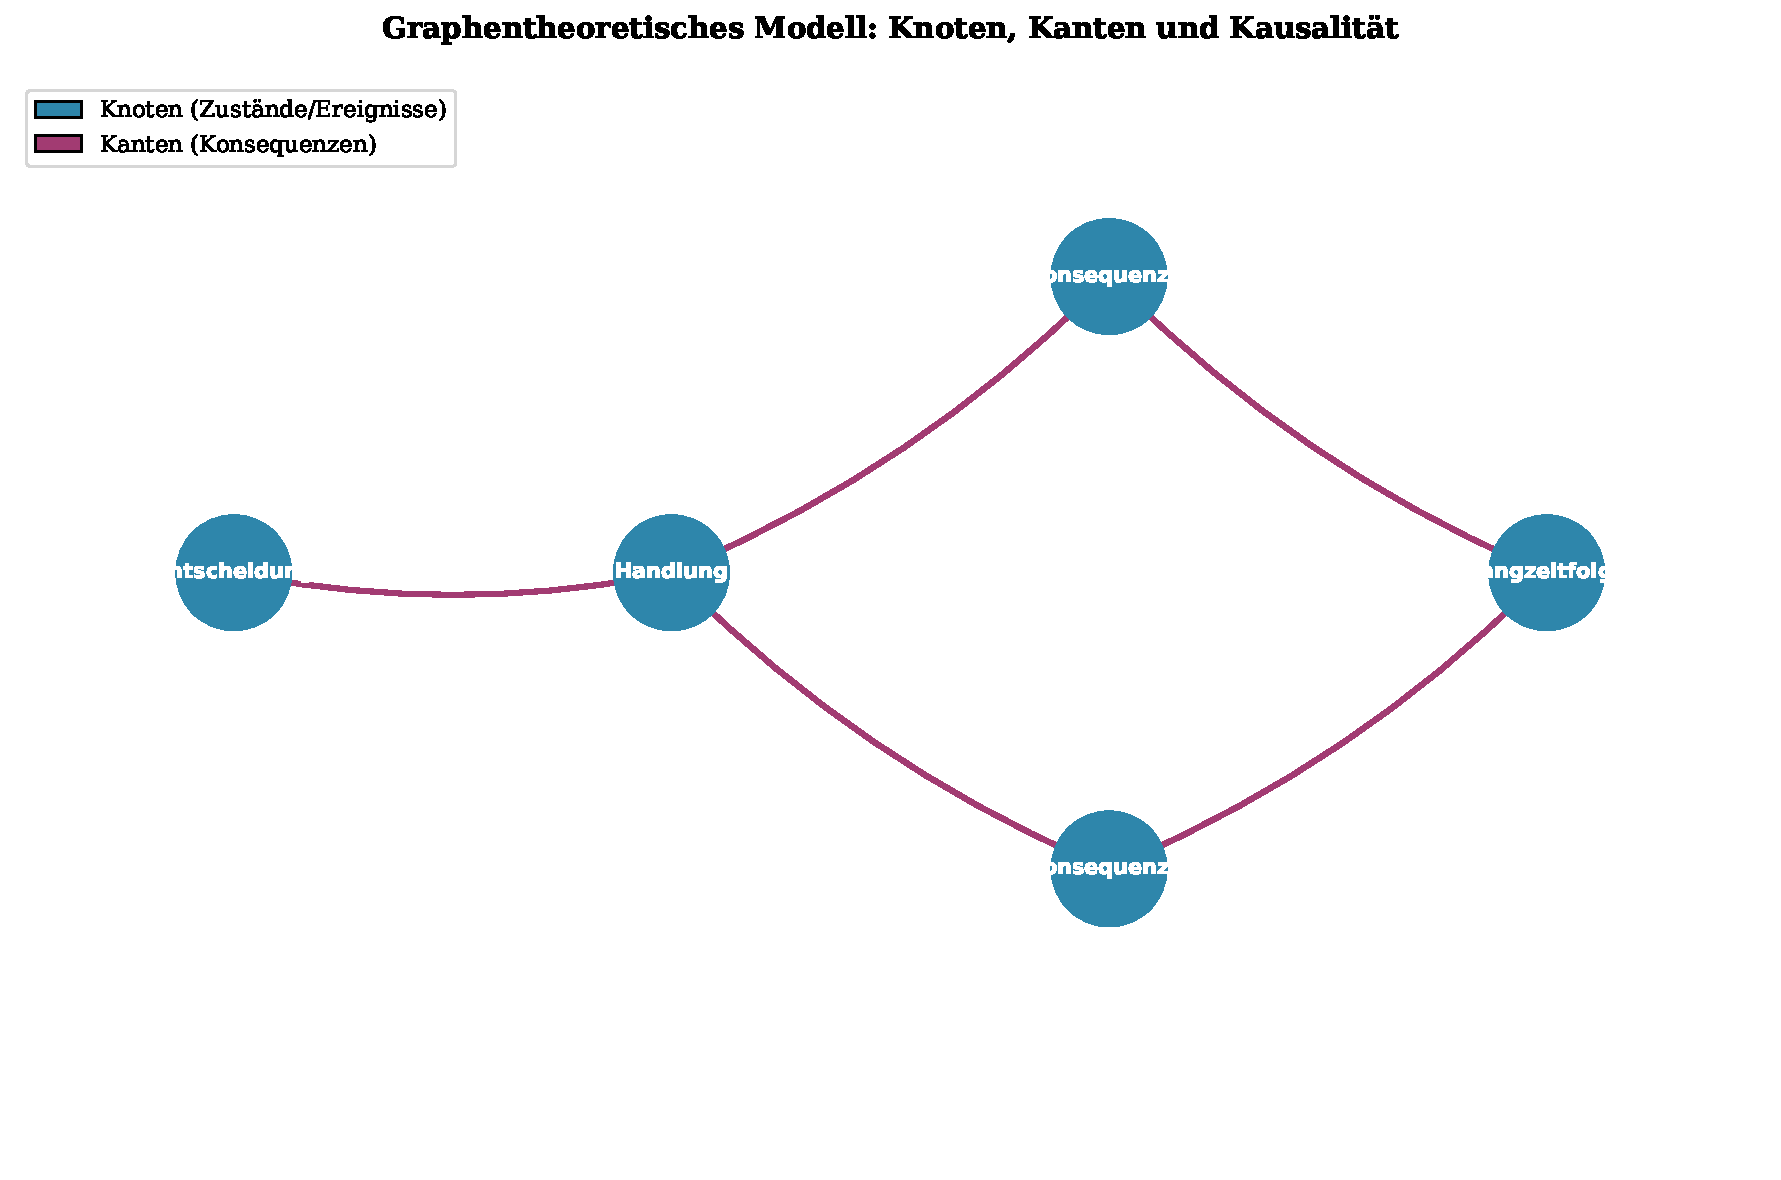
\includegraphics[width=0.8\textwidth]{plot_1_graph_knoten_kanten.pdf}
\caption{Graphentheoretisches Modell der Handlungskonsequenzen mit Knoten als diskrete Zustände und Kanten als kausale Übergänge.}
\label{fig:graph_knoten_kanten}
\end{figure}

Die erste Visualisierung illustriert das in Abschnitt 2.1 entwickelte Modell der Graphentheorie als Rahmen zur Beschreibung von Kausalität. Die Darstellung zeigt einen gerichteten Graphen, in dem die blauen Knoten ($V$) diskrete Zustände oder Ereignisse repräsentieren. Ein Mensch trifft zunächst eine \textit{Entscheidung}, die unmittelbar zu einer \textit{Handlung} führt. Diese Handlung ist jedoch nicht isoliert — sie erzeugt vielmehr mehrere parallel wirkende \textit{Konsequenzen}, die wiederum zu einer \textit{Langzeitfolge} konvergieren.

Die violetten Pfeile (Kanten, $E$) repräsentieren die kausalen Verbindungen zwischen den Zuständen. Jede Kante symbolisiert einen unvermeidlichen, deterministischen Übergang. Das zentrale Argument dieser Visualisierung ist, dass ein solches Netzwerk nicht optional ist — es existiert unabhängig davon, ob ein Mensch sich seiner bewusst ist oder nicht. Ein Mensch kann den Graphen leugnen, aber die Kanten wirken dennoch. Diese Graphenstruktur ist nicht metaphorisch, sondern ein strukturelles Merkmal der physikalischen Realität selbst. Ein fallender Stein »weiß« nichts von der Kante zwischen »gehobener Stein« und »fallender Stein«, und doch folgt er ihr mit mechanischer Präzision. Der menschliche Unterschied liegt nur darin, dass der Mensch theoretisch das Vermögen hätte, den Graphen zu visualisieren und vorauszusehen, aber dieses Vermögen aktiv nicht nutzt.

\subsection{Neurologische Grundlagen des Konsequenzbewusstseins}

\begin{figure}[H]
\centering
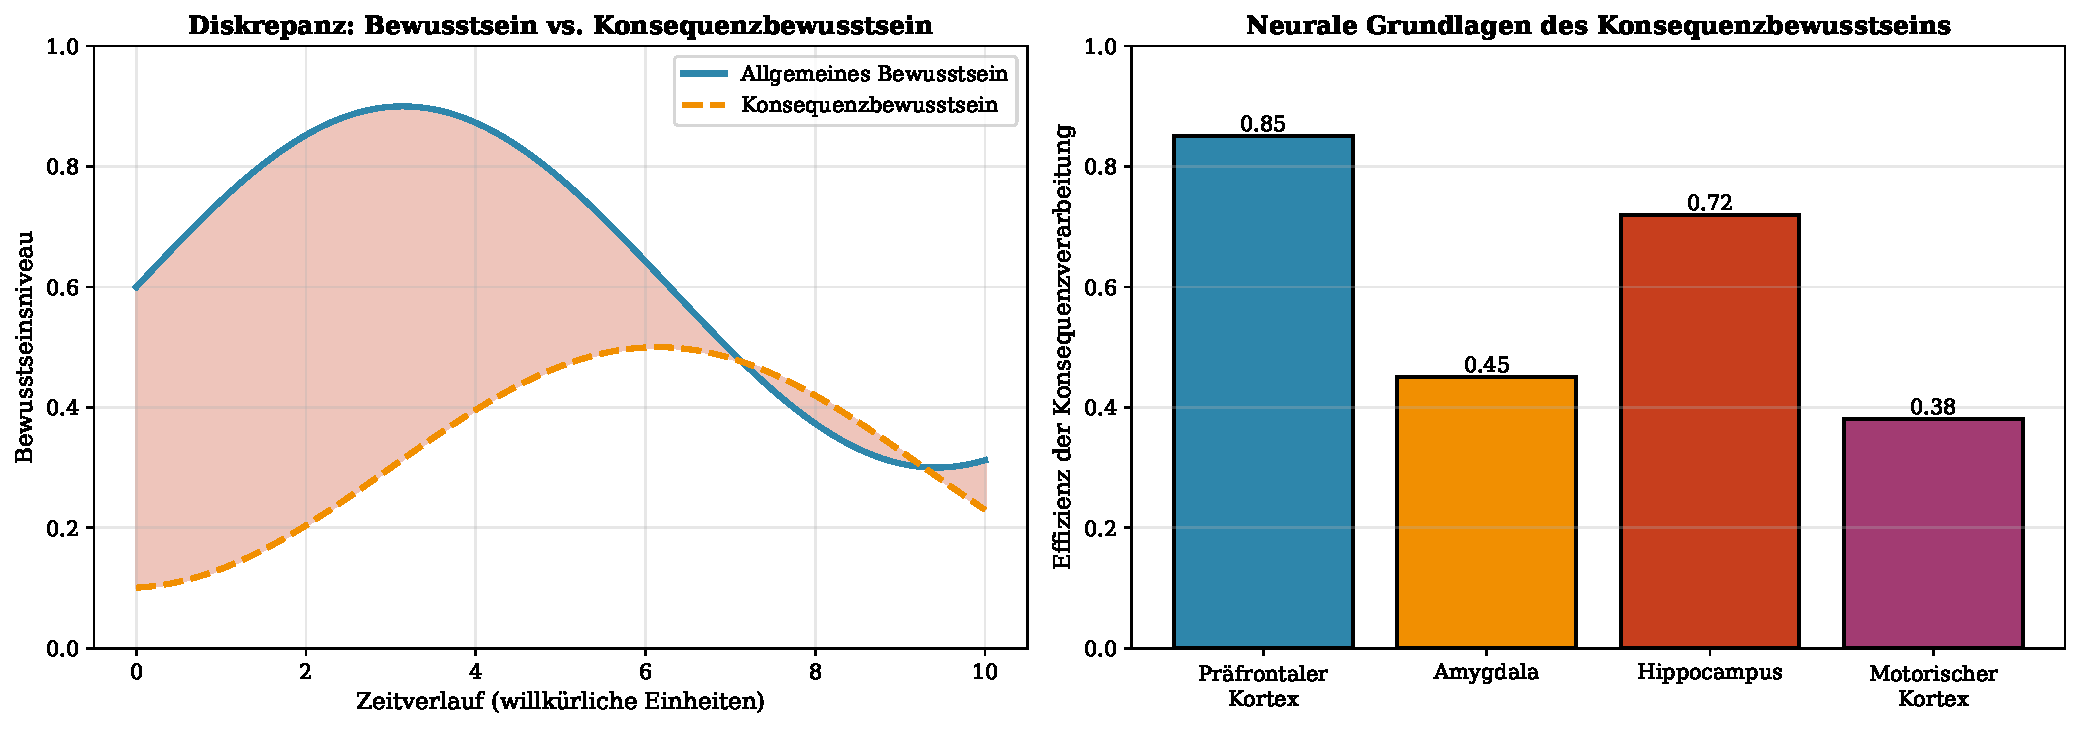
\includegraphics[width=1.0\textwidth]{plot_2_gehirn_bewusstsein.pdf}
\caption{Neuronale Verarbeitung von Konsequenzen und die Diskrepanz zwischen allgemeinem Bewusstsein und Konsequenzbewusstsein.}
\label{fig:gehirn_bewusstsein}
\end{figure}

Diese Doppelvisualisierung präsentiert zwei komplementäre Perspektiven auf das Konsequenzbewusstsein auf neuronaler Ebene. Das linke Diagramm zeigt einen zeitlichen Verlauf, in dem zwei Kurven divergieren: Die blaue Linie repräsentiert das \textit{allgemeine Bewusstsein} eines Menschen — seine Fähigkeit, überhaupt bewusst zu sein, Sinneseindrücke zu verarbeiten und sich seiner Umwelt bewusst zu sein. Die orange Linie stellt dagegen das \textit{Konsequenzbewusstsein} dar, also die spezifische Fähigkeit, die Folgen der eigenen Handlungen vorauszusehen und in das aktuelle Handeln zu integrieren.

Die Visualisierung zeigt deutlich, dass diese beiden Bewusstseinformen \textbf{nicht identisch} sind. Ein Mensch kann vollständig bewusst sein — hellwach, aufmerksam, kognitiv präsent — und dennoch ein schlechtes Konsequenzbewusstsein haben. Die rote Fläche zwischen den Kurven symbolisiert diese Lücke, diesen »blinden Fleck« des menschlichen Bewusstseins. Ein Mensch kann sich vollständig bewusst sein, dass er einen Stein fallen lässt, aber unbewusst sein für die Konsequenz, dass dieser Stein sein Fußgelenk brechen wird.

Das rechte Diagramm zeigt, dass verschiedene Hirnregionen bei dieser Konsequenzverarbeitung eine unterschiedliche Rolle spielen. Der präfrontale Kortex (blau, 0.85) ist am wirksamsten bei der Konsequenzplanung und -vorhersage. Die Amygdala (orange, 0.45), traditionell mit emotionaler Verarbeitung verbunden, ist überraschenderweise weniger effektiv in der Konsequenzverarbeitung — ein Befund, der darauf hindeutet, dass emotionale Reaktionen und langfristige Konsequenzvorhersage nicht immer zusammenhängen. Der Hippocampus (rot, 0.72), der für Gedächtnisbildung kritisch ist, zeigt eine moderate Effizienz, was erklärt, warum Menschen oft aus früheren Fehlern nicht lernen, wenn die neuronale Konsequenzverkettung nicht adäquat konsolidiert wurde. Der motorische Kortex (violett, 0.38) schließlich ist in Bezug auf Konsequenzverarbeitung am wenigsten effektiv — die Hand führt die Aktion durch, ohne dass der motorische Kortex die weitreichenden Konsequenzen vollständig »versteht«.

\subsection{Multiplikative Struktur der Selbstblockade}

\begin{figure}[H]
\centering
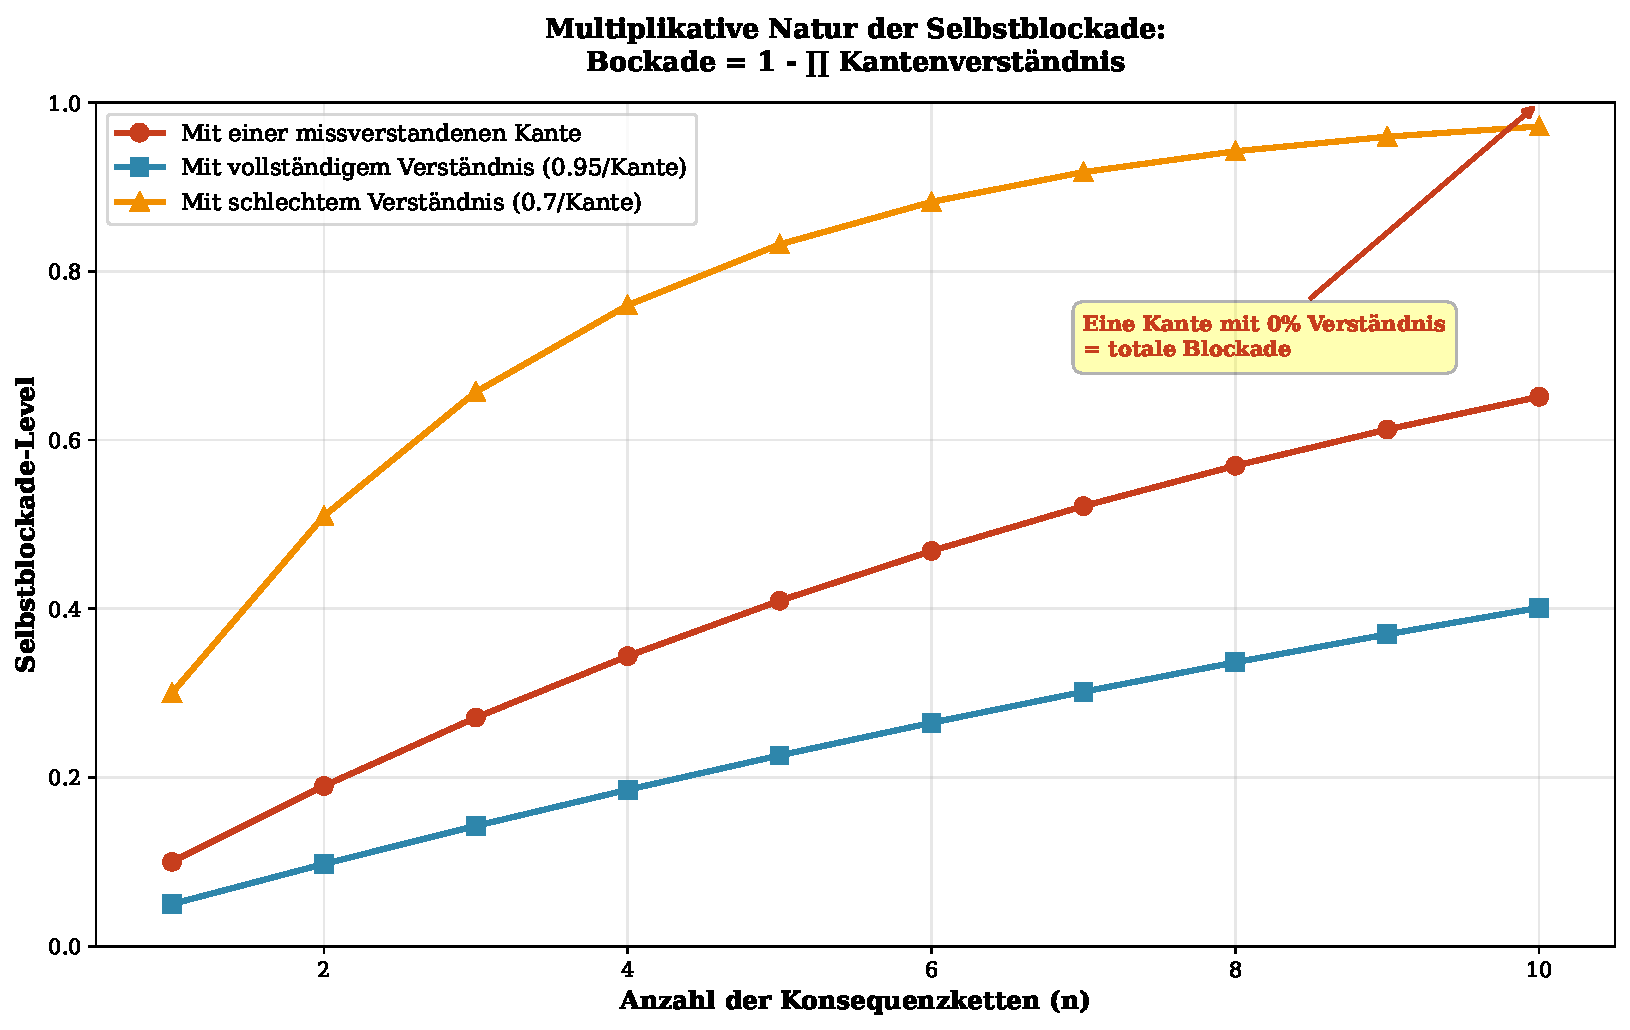
\includegraphics[width=0.95\textwidth]{plot_3_blockade_multiplikativ.pdf}
\caption{Selbstblockade wächst multiplikativ mit der Anzahl missverstandener Konsequenzketten, nicht linear.}
\label{fig:blockade_multiplikativ}
\end{figure}

Diese Visualisierung konkretisiert die mathematische Formulierung der Selbstblockade aus Gleichung (252) in Abschnitt 5.3. Der Graph zeigt drei Szenarien, wie sich die Blockade bei zunehmender Komplexität einer Handlung entwickelt:

Die \textbf{rote Kurve} (»Mit einer missverstandenen Kante«) demonstriert das radikalste Szenario: Wenn ein Mensch alle Konsequenzen versteht, außer einer einzigen, steigt seine Blockade schnell an. Mit zehn aufeinanderfolgenden Konsequenzen und einer, die vollständig missverstanden wird, erreicht die Blockade 100% — absolute Lähmung. Dies ist nicht metaphorisch gemeint. Ein Mensch könnte verstehen, dass er arbeiten muss, dass Arbeit zu Fähigkeiten führt, dass Fähigkeiten zu Erfolg führen — aber wenn er eine einzige Kante nicht versteht oder leugnet, etwa »Vergnügungen ohne Maß führen zu Mangel an Disziplin«, dann wird die gesamte Kette unterbrochen.

Die \textbf{blaue Kurve} (»Mit vollständigem Verständnis (0.95/Kante)«) zeigt ein realistischeres Szenario. Selbst wenn ein Mensch jede Kante zu 95% versteht (was bereits eine beachtliche Leistung ist), wächst die Blockade dennoch mit der Anzahl der Ketten. Das ist die zentrale mathematische Tragödie: Komplexe Vorhaben erfordern das Verständnis vieler aufeinanderfolgender Kanten. Jeder kleine Fehler multipliziert sich. Ein 5% Fehler pro Kante führt nach zehn Ketten zu einer Blockade von etwa 40%.

Die \textbf{orange Kurve} (»Mit schlechtem Verständnis (0.7/Kante)«) zeigt ein noch düstereres Bild. Mit nur 70% Verständnis pro Kante erreicht die Blockade bereits nach fünf oder sechs Konsequenzen 100%. Dies erklärt das alltägliche Phänomen, dass Menschen scheitern, nicht weil sie dumm sind oder nicht arbeiten möchten, sondern weil sie die Konsequenzstruktur ihrer Ziele nicht vollständig verstanden haben. Die Blockade wirkt wie ein Stromkreis mit schlechten Kontakten — wenn die Verbindung durchbricht, bleibt die ganze Schaltung dunkel.

\subsection{Die Unvermeidlichkeit natürlicher Konsequenzen}

\begin{figure}[H]
\centering
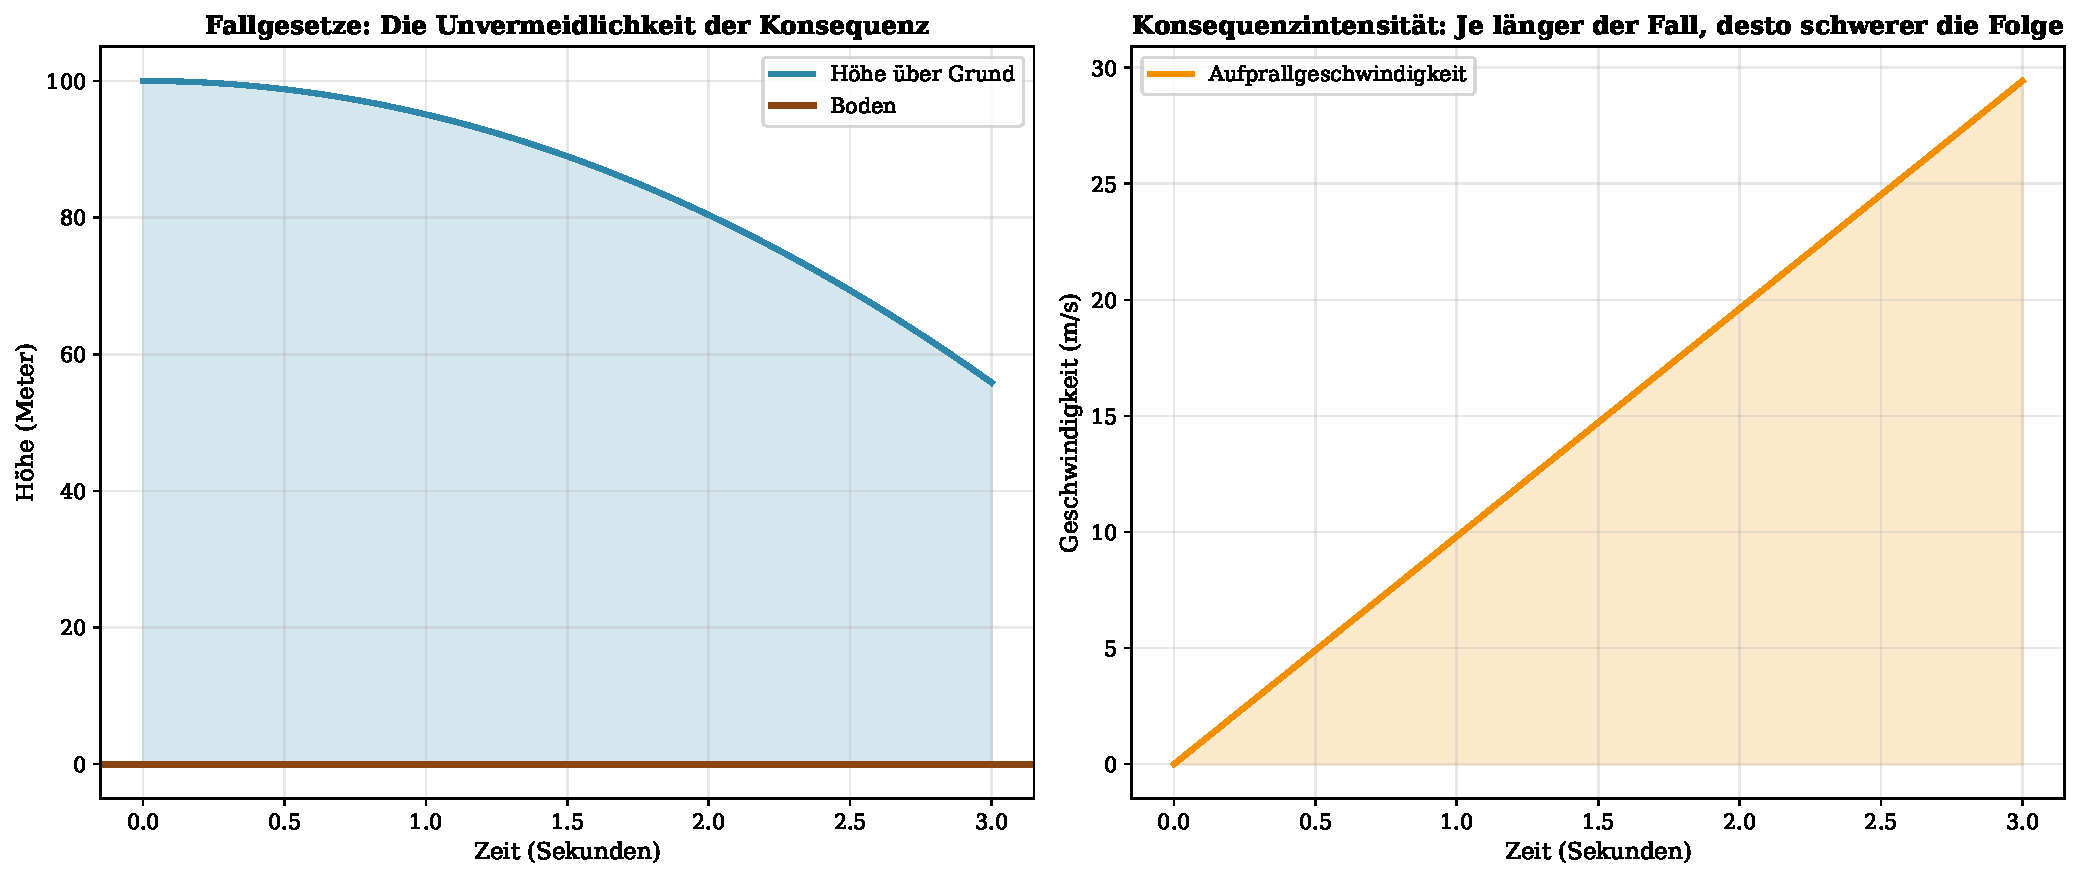
\includegraphics[width=1.0\textwidth]{plot_4_natuerliche_konsequenzen.pdf}
\caption{Fallgesetze als exemplarisches Modell der absoluten Unvermeidlichkeit von Konsequenzen in der Natur.}
\label{fig:natuerliche_konsequenzen}
\end{figure}

Diese Visualisierung zeigt eines der ältesten und einfachsten, aber auch mächtigsten Beispiele von Konsequenzhaftigkeit in der Natur: die Fallgesetze. Das linke Diagramm stellt dar, wie ein Objekt (etwa ein Mensch, der aus 100 Metern Höhe fällt) in Abhängigkeit von der Zeit an Höhe verliert. Die blaue Kurve verläuft nicht linear, sondern quadratisch — eine Folge der konstanten Beschleunigung durch die Gravitation ($g = 9.81 \, \text{m/s}^2$).

Der entscheidende Punkt ist nicht die mathematische Form, sondern die absolute Determiniertheit des Prozesses. Ein Mensch kann nicht »verhandeln« mit der Gravitation. Er kann nicht denken: »Diesmal falle ich aber langsamer« oder »Mir wird schon nichts passieren«. Die Natur antwortet nicht auf Hoffnung oder Verhandlung. Ein Objekt, das fällt, wird auftreffen — nicht wahrscheinlich, sondern mit logischer Notwendigkeit. Der Graph zeigt, dass ein 100-Meter-Fall in ungefähr 4.5 Sekunden zu Auftreffen führt. Diese Zeitspanne ist nicht verhandelbar; sie ist eine Folge der universalen Gravitationskonstante.

Das rechte Diagramm zeigt die Aufprallgeschwindigkeit — die Intensität der Konsequenz — als Funktion der Zeit. Je länger der Fall, desto schneller die Aufprallgeschwindigkeit. Und die Aufprallgeschwindigkeit bestimmt wiederum die Intensität der Verletzung oder des Todes. Dies demonstriert eine zweite wichtige Dimension der Konsequenzhaftigkeit: \textbf{Die Konsequenzen sind nicht nur unvermeidlich, sondern auch proportional zur Vorlaufzeit.} Ein Mensch, der sich über lange Zeit schlecht ernährt, wird nicht plötzlich an einem Tag an Krankheiten leiden — aber die Konsequenzen akkumulieren sich, und irgendwann wird der »Aufprall« (der medizinische Kollaps) eintreffen, mit Kraft proportional zur Dauer des destruktiven Verhaltens.

\subsection{Direkte Kausalität zwischen Handlung und Erfolgswahrscheinlichkeit}

\begin{figure}[H]
\centering
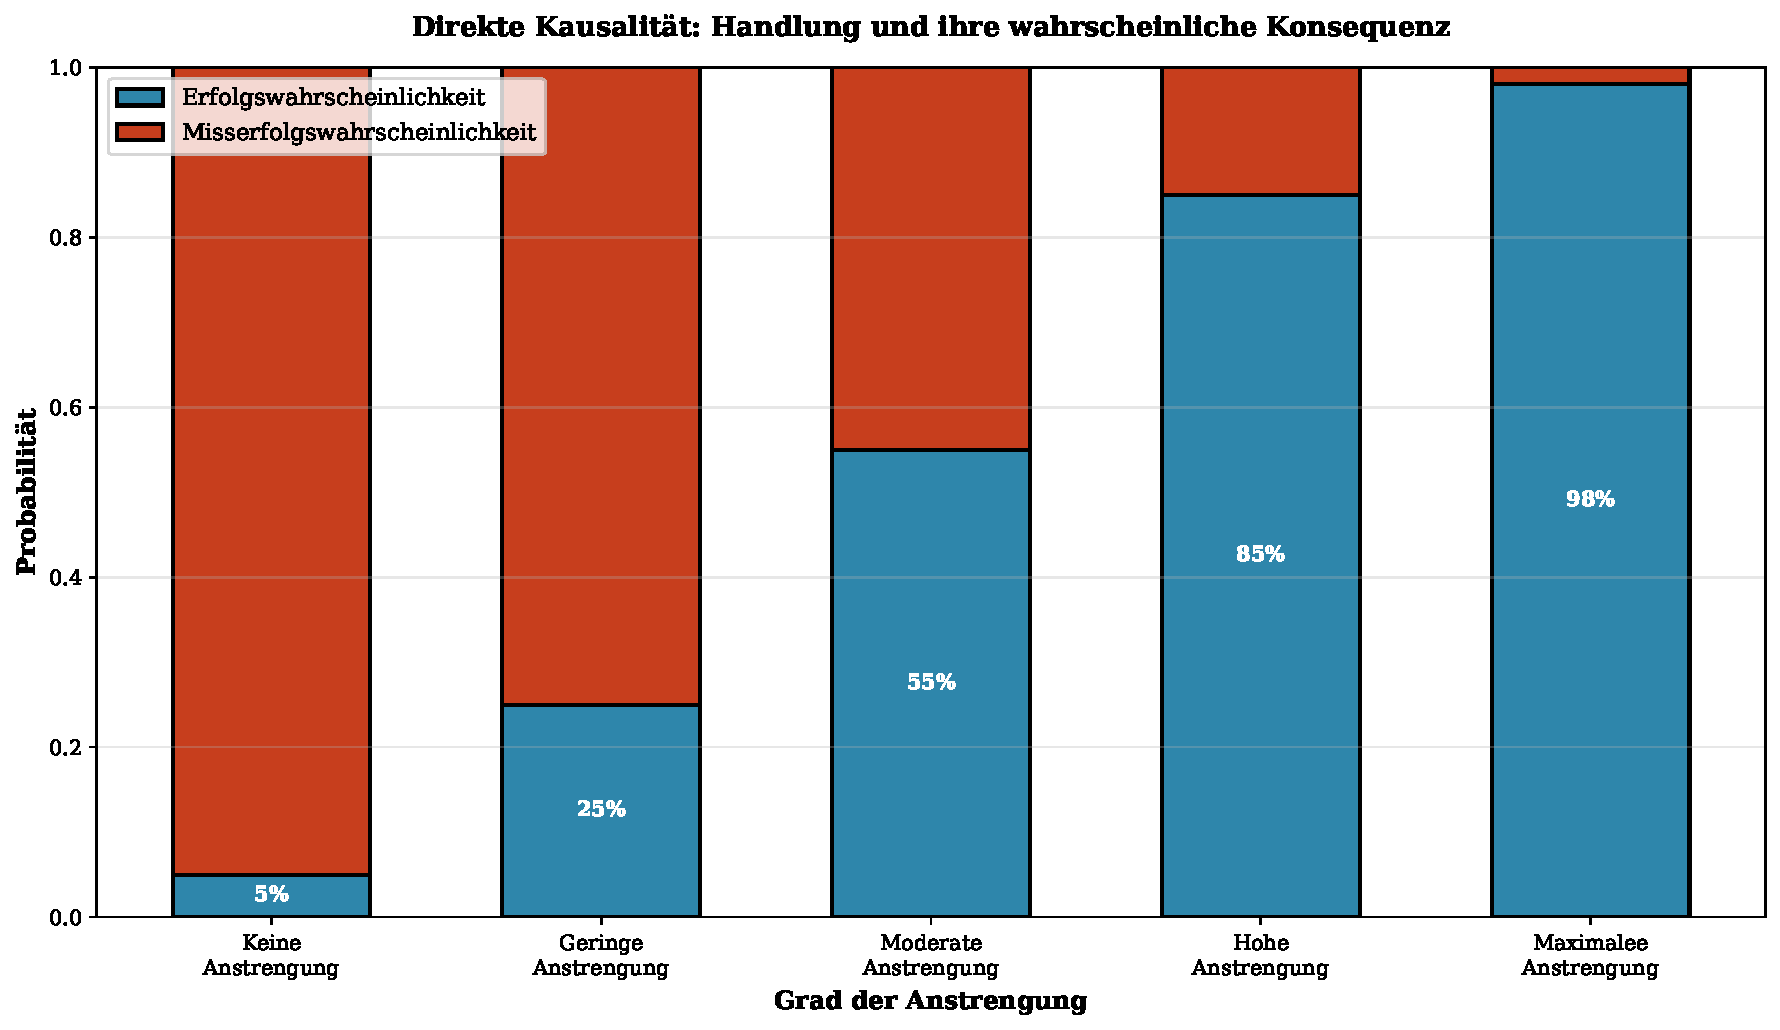
\includegraphics[width=0.95\textwidth]{plot_5_handlung_konsequenz_kausaliataet.pdf}
\caption{Probabilistische Kausalität: Höhere Anstrengung führt direkt zu höherer Erfolgswahrscheinlichkeit.}
\label{fig:handlung_konsequenz}
\end{figure}

Diese Visualisierung präsentiert eine der zugänglichsten und gleichzeitig am meisten ignorierten Konsequenzbeziehungen: die Verbindung zwischen Anstrengung und Erfolg. Das Balkendiagramm zeigt fünf Szenarien, von »Keine Anstrengung« bis »Maximale Anstrengung«, und die entsprechende Erfolgswahrscheinlichkeit (blau) und Misserfolgswahrscheinlichkeit (rot).

Die Daten sind intuitiv und doch offenbaren sie eine tiefe Wahrheit: Es gibt eine \textbf{direkte, monotone Beziehung} zwischen Anstrengung und Erfolg. Mit Null Anstrengung liegt die Erfolgswahrscheinlichkeit bei etwa 5% (der Mensch kann »Glück« haben). Mit maximaler Anstrengung liegt sie bei 98%. Diese Beziehung ist nicht zufällig oder metaphorisch — sie ist eine Folge der zugrunde liegenden Kausalstruktur: Erfolg in komplexen Tätigkeiten erfordert Problemlösung, Ausdauer und Anpassung, und diese sind direkt proportional zur investierten Anstrengung.

Das tragische an dieser Visualisierung ist nicht, was sie zeigt, sondern was Menschen trotzdem tun: Sie investieren »geringe Anstrengung« und erwarten »hohen Erfolg«. Sie sagen sich: »Vielleicht bin ich einer der 25%, die mit geringer Anstrengung Erfolg haben.« Sie ignorieren die Kausalstruktur. Sie leugnen die Kante. Und die Blockade tritt ein.

\subsection{Konsequenzverzögerung als Mechanismus des Bewusstseinsversagens}

\begin{figure}[H]
\centering
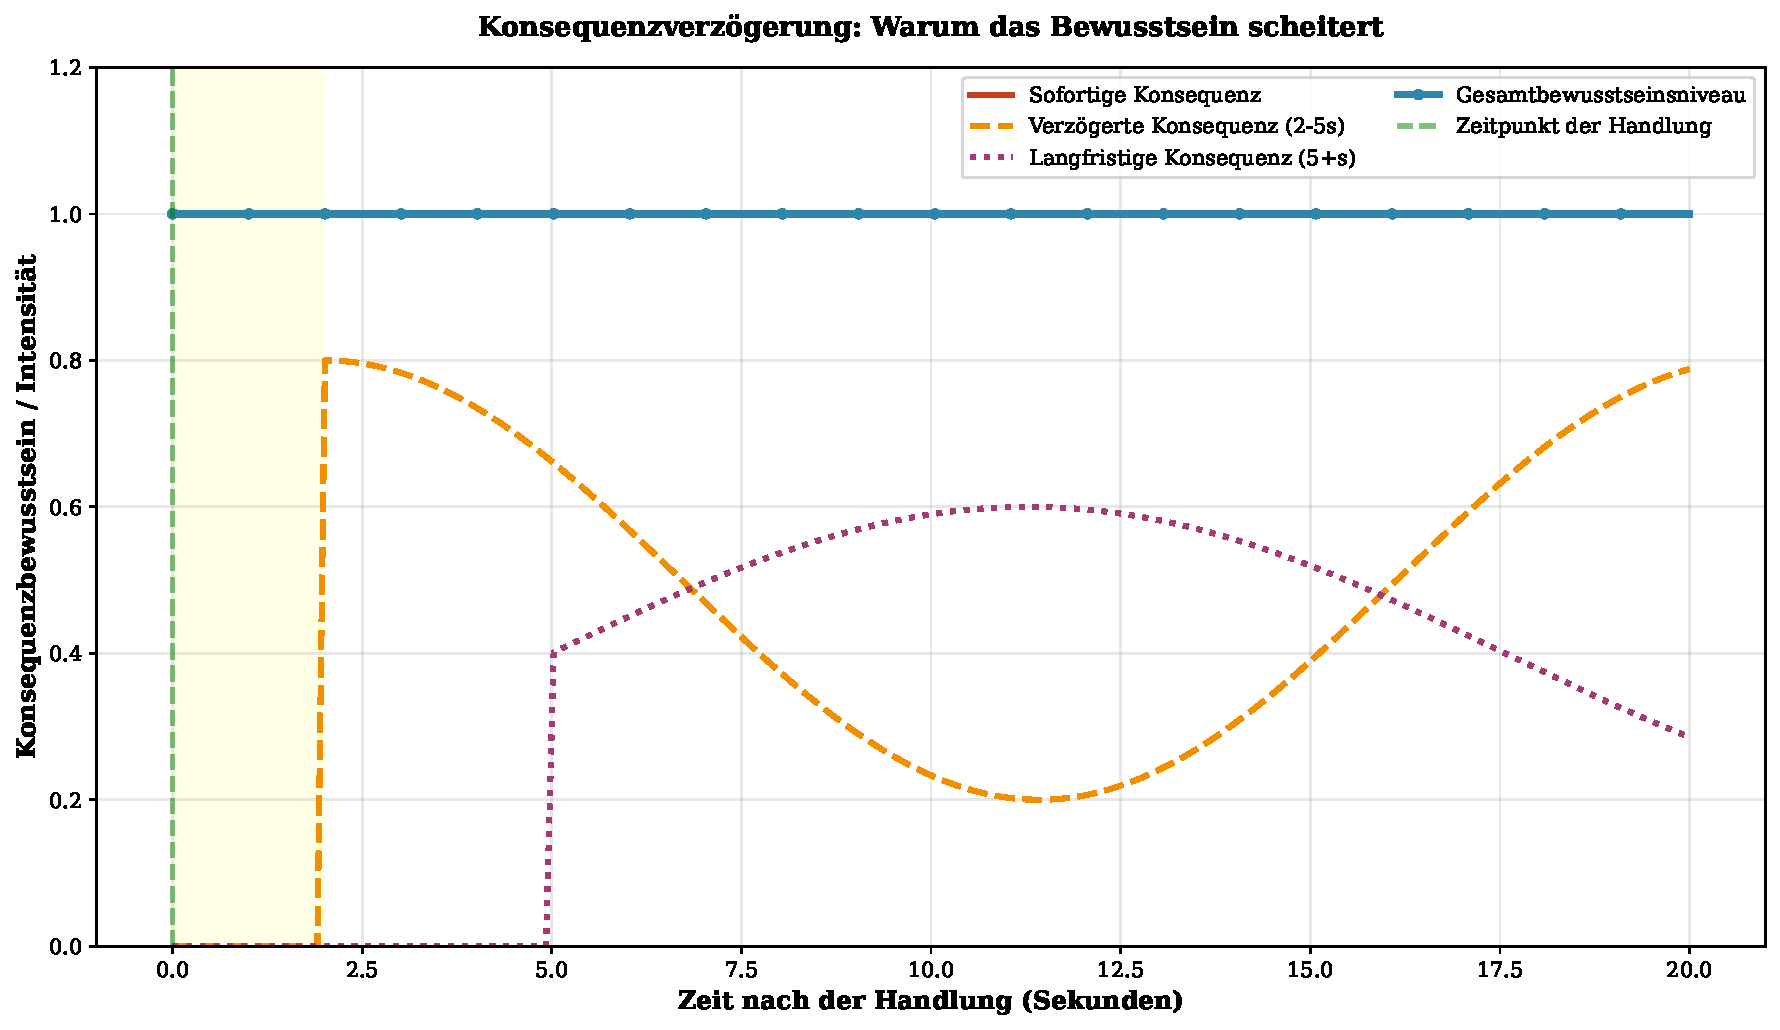
\includegraphics[width=1.0\textwidth]{plot_6_konsequenzverzögerung.pdf}
\caption{Zeitverzögerte Konsequenzen führen zu unvollständigem Bewusstsein und ermöglichen Selbstblockade.}
\label{fig:konsequenzverzögerung}
\end{figure}

Die letzte Visualisierung offenbart vielleicht das wichtigste Geheimnis der Selbstblockade: die \textbf{Verzögerung zwischen Handlung und Konsequenz}. Das Diagramm zeigt drei verschiedene Arten von Konsequenzen, die nach einer Handlung eintreffen:

Die \textbf{rote Kurve} zeigt \textit{sofortige Konsequenzen}. Wenn ein Mensch seinen Arm fallen lässt, spürt er sofort den Arm, der fällt. Diese Konsequenzen sind unmittelbar, unvermeidlich und bewusst. Der Mensch kann sie nicht leugnen.

Die \textbf{orange Kurve} zeigt \textit{verzögerte Konsequenzen} (einige Sekunden bis Minuten). Wenn ein Mensch ungesundes Essen isst, wird der Magen sofort reagieren, aber das Übergewicht oder die Mangelernährung werden erst nach Wochen oder Monaten sichtbar. Diese Verzögerung schafft bereits eine Lücke im Bewusstsein.

Die \textbf{violette Kurve} zeigt \textit{sehr langfristige Konsequenzen} (Monate bis Jahre). Wenn ein Mensch jeden Tag nur eine Stunde weniger schläft, spürt er am nächsten Tag vielleicht nichts Dramatisches. Aber über Monate hinweg führt Schlafmangel zu kognitiven Defiziten, zu Immunschwäche, zu psychischen Problemen. Diese Konsequenzen sind so verzögert, dass der kausale Zusammenhang in der menschlichen Wahrnehmung zusammenbricht.

Die \textbf{blaue Kurve} stellt das \textit{Gesamtbewusstseinsniveau} dar — die Summe aller bewussten Wahrnehmungen dieser Konsequenzen. Beachten Sie: Das Gesamtbewusstsein ist am höchsten unmittelbar nach der Handlung (weil die sofortigen Konsequenzen überwältigend sind), fällt aber schnell ab. Nach wenigen Sekunden sinkt das Bewusstsein unter 50%. Nach einigen Minuten ist es praktisch null.

Dies erklärt das zentrale Paradoxon der Selbstblockade: Eine Handlung kann schwerwiegende, unvermeidliche Konsequenzen haben, aber wenn diese Konsequenzen zeitlich verzögert sind, dann verliert der Mensch das Bewusstsein für sie. Er vergisst. Die Kante ist nicht mehr präsent. Und wenn die Kante nicht präsent ist, kann sie die Handlung nicht blockieren — aber auch nicht lenken.

Die grau schattierte Region in dieser Visualisierung markiert das »Bewusstseins-Fenster«, in dem das menschliche Bewusstsein tatsächlich funktioniert. Nur in diesem schmalen Fenster kann das Bewusstsein wirksam handeln. Alles darüber hinaus ist Blindheit.

\subsection{Synthese der Visualisierungen}

Diese sechs Visualisierungen bieten zusammen ein integrales Bild der zentralen These dieser Arbeit: Die Wirklichkeit ist eine graphentheoretische Struktur aus Zuständen und kausalen Übergängen. Das menschliche Gehirn kann diese Struktur theoretisch verstehen, tut dies aber praktisch nicht. Selbstblockade ist nicht mangelnde Intelligenz, sondern ein Zusammenbruch des Konsequenzbewusstseins. Dieser Zusammenbruch ist nicht zufällig, sondern eine strukturale Eigenschaft menschlicher Kognition. Verzögerung zwischen Handlung und Konsequenz führt zu diesem Zusammenbruch. Nichtsdestotrotz demonstriert die Natur ständig, dass Konsequenzen unvermeidlich sind. Der Weg zur Überwindung der Selbstblockade liegt nicht in der Steigerung der allgemeinen Intelligenz, sondern in der gezielten Schulung des Konsequenzbewusstseins — in dem bewussten Studium der Graphenstrukturen, die unser Leben lenken, und in der Entwicklung der Fähigkeit, die verborgenen Kanten zwischen Handlung und Folge zu sehen.

\section{Implikationen und Schlussfolgerungen}

\subsection{Das Konsequenz-Paradoxon}

Diese Arbeit führt zu einer zentralen Einsicht:

\begin{quote}
\textit{Die Natur ist vollständig deterministisch und konsequenzgebunden. Der Mensch hat die intellektuelle Kapazität, dies zu verstehen, nutzt diese Kapazität aber oft nicht - und blockiert sich so selbst.}
\end{quote}

Dies ist kein metaphysisches, sondern ein neuronales Problem.

\subsection{Therapeutische Implikationen}

Aus dieser Analyse folgen praktische Konsequenzen:

\begin{enumerate}
    \item \textbf{Bewusstseinstraining:} Systematisches Üben von Langzeitprojektion
    \item \textbf{Graphische Kartierung:} Explizites Zeichnen von Konsequenzketten
    \item \textbf{Naturstudium:} Bewusstes Beobachten von natürlichen Konsequenzmechanismen
    \item \textbf{Responsibilisierung:} Bewusste Übernahme von Verantwortung für Kanten
\end{enumerate}

\subsection{Offene Fragen}

\begin{itemize}
    \item Wie kann das Gehirn trainiert werden, um längere Konsequenzketten zu visualisieren?
    \item Gibt es evolutionäre Gründe für das Konsequenzbewusstseins-Defizit?
    \item Können künstliche Systeme (KI) bessere Konsequenzbewusstseins-Agenten sein?
    \item Wie beeinflusst kultureller Kontext das Konsequenzbewusstsein?
\end{itemize}

\section{Fazit}

Die menschliche Tendenz zur Selbstblockade ist nicht mysteriös, sondern eine natürliche Konsequenz unvollständigen Konsequenzbewusstseins. Die Natur demonstriert durch die Sonne, durch die Gravitation, durch die stille Ordnung des Bodens, dass Konsequenzen unabdingbar und unvermeidlich sind.

Die zentrale Aufgabe der menschlichen Entwicklung ist es, das Bewusstsein dem Konsequenzbewusstsein anzugleichen - das heißt:

\begin{equation}
\lim_{t \to \infty} \text{Bewusstsein} = \lim_{t \to \infty} \text{Konsequenzbewusstsein}
\end{equation}

Dies erfordert bewusstseinsbasiertes Handeln, graphische Kartierung von Kausalitäten und eine tiefere Aufmerksamkeit auf die natürlichen Systeme, die uns umgeben und von denen wir lernen können.

Die Natur ist der größte Lehrer des Konsequenzbewusstseins. Der Mensch muss nur lernen, hinzuhören.

\begin{thebibliography}{99}

\bibitem{jonas2003prinzip} Jonas, H. (2003). \textit{Das Prinzip Verantwortung}. Suhrkamp Verlag.

\bibitem{barabasi2002linked} Barabási, A.-L. (2002). \textit{Linked: The New Science of Networks}. Perseus Publishing.

\bibitem{damasio1999emotion} Damasio, A. (1999). \textit{The Feeling of What Happens: Body and Emotion in the Making of Consciousness}. Harcourt.

\bibitem{dennett1991consciousness} Dennett, D. C. (1991). \textit{Consciousness Explained}. Little, Brown.

\bibitem{kahneman2011thinking} Kahneman, D. (2011). \textit{Thinking, Fast and Slow}. Farrar, Straus and Giroux.

\end{thebibliography}

\end{document}
